

\documentclass[fleqn]{article}


\usepackage[margin = 1in,includefoot]{geometry} 
\usepackage{amsmath}
\usepackage{amssymb}
\usepackage{stix}
\usepackage{amsthm}
\usepackage{graphicx}
 \usepackage{tikz}
 \usepackage{hyperref}
\usepackage{parskip}
\graphicspath{ {./kakes_pics/} }


\newcommand{\FIG}[2]{
 \begin{figure}[!hbt]
 \begin{center}
 \begin{minipage}{0.85\textwidth}
 \centering{\includegraphics[width=90mm]{#1}}
 \caption{\label{#1}\small{#2}}
 \end{minipage}
 \end{center}
 \end{figure}
 }


\newcommand{\3}{\vspace*{3mm}}

\title{Life in the Sovereign Kingdom of Kakesland}
\author{Rishab Bomma}

\newcommand{\Kakes}{S.K.K \hspace*{.15mm}}

 \setlength{\parindent}{0mm}
\setlength{\parskip}{1mm}

\begin{document}



\pagenumbering{gobble}
 \maketitle
  \FIG{INTRO}{Der schlimmste Feind deiner Mutter}
\newpage
\pagenumbering{arabic}

\section*{Kakesland: Is it a Punk Rock Band?}



\hspace*{3mm}The Sovereign Kingdom of Kakesland or as I will refer to it the \Kakes is a country who I, Rishab Bomma was invited to, for the purpose of reporting on the people, and life there in general. To my dismay the \Kakes was not a punk rock band, and I was not being invited to their yacht. I was instead expected to learn more about their culture, while not exactly dull was quite exaggerated. But don't let my non-enthusiastic voice turn you off from the \Kakes. Let their lies, methods of deception and in my opinion outright disrespect of their constituents disgust you.

\3

\3

 \begin{figure}[!hbt]
 \begin{center}
 \begin{minipage}{0.85\textwidth}
 \centering{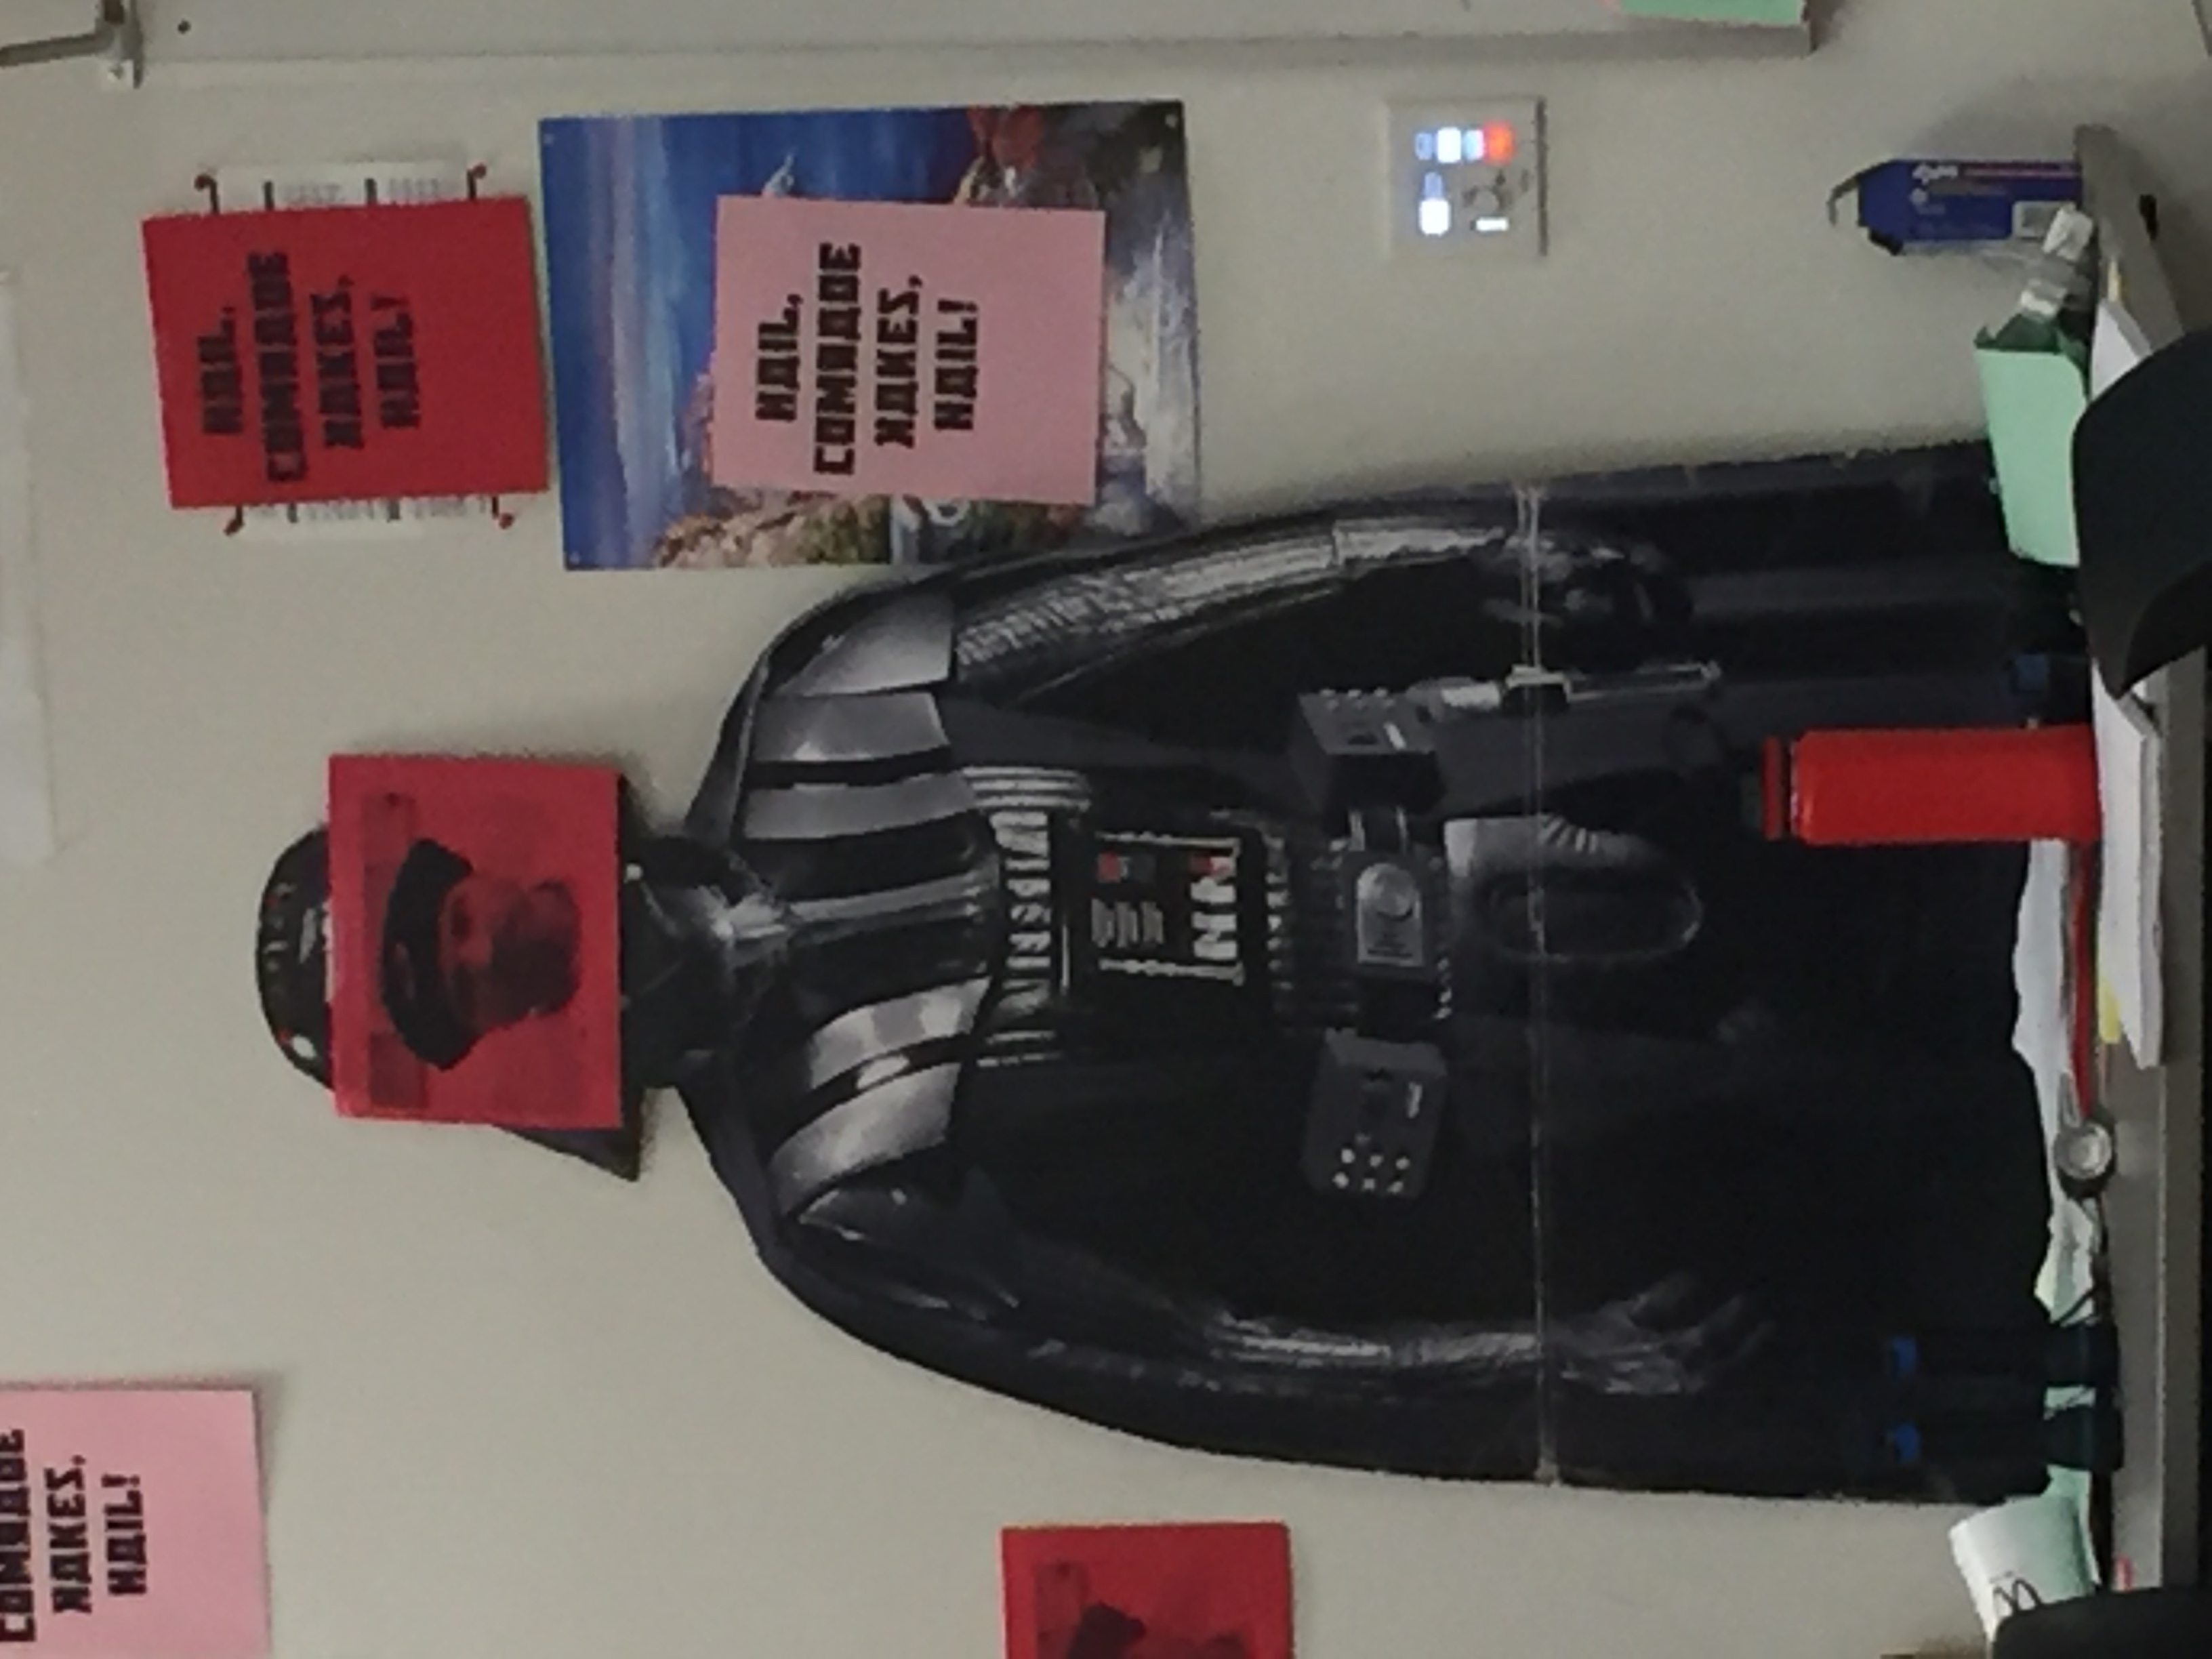
\includegraphics[width=90mm, angle=270]{MIDDLE}}
 \caption{\label{MIDDLE}\small{The defacement of Darth Vader with the disgusting jawline of the leader of Kakesland, Mr.Kakes }}
 \end{minipage}
 \end{center}
 \end{figure}

\subsection*{Worker Rights? Texas or California? }

\3

The \Kakes is quite a questionable source, and while one must learn about my findings it is useful to put them in perspective. The following sections of my article are to show how the disgusting Mr.Kakes misinforms the world around him, about the "great" S.K.K. He frames his society as "Prosperous" even though my findings suggest otherwise. Anyway, labor rights are quite fair to workers everywhere in Kakesland according to Mr.Kakes. While at the same time they have accomplished their economic goals, similar to that of the $5$ year plan created by Stalin to industrialize the USSR. Simultaneously, having the most advanced tech and machinery in the entire world. 


\3

\subsection*{Arts and Culture}

\3

Arts and Culture in Kakesland are said to be very prosperous. All artists are encouraged to push their own boundaries, and censorship concerning art has never occurred. Kakesland has also been a hotspot of artistic accomplishment. According to Mr.Kakes himself, Kakesland should be considered the "Belushi of the World" in the context of art. I have not yet concluded the validity of his claim, or if he even understands what it means but I take it that he is very proud of the art his country's artists produce. 

\3

\subsection*{Anna Howard Shaw? Putin?}

\3

Women's rights in Kakesland are said to be really strong, and in his own words "Women have been valued since 1917". Now if Mr.Kakes was sarcastic is still quite unclear but along with that somewhat worrying statement women have the ability to join the military. And in general are considered to be equal to everyone else. Women have the option of going to university and can receive and education. 

\3

\subsection*{Anthony Weiner? Bernie Sanders? Trump?}

\3

According to Mr.Kakes everyone in Kakesland has the option to choose to vote for whoever they want. They are not ever forced or coerced to vote for his party or anyone else's. The validity of these statements thought are not set in stone.

\3

 \begin{figure}[!hbt]
 \begin{center}
 \begin{minipage}{0.85\textwidth}
 \centering{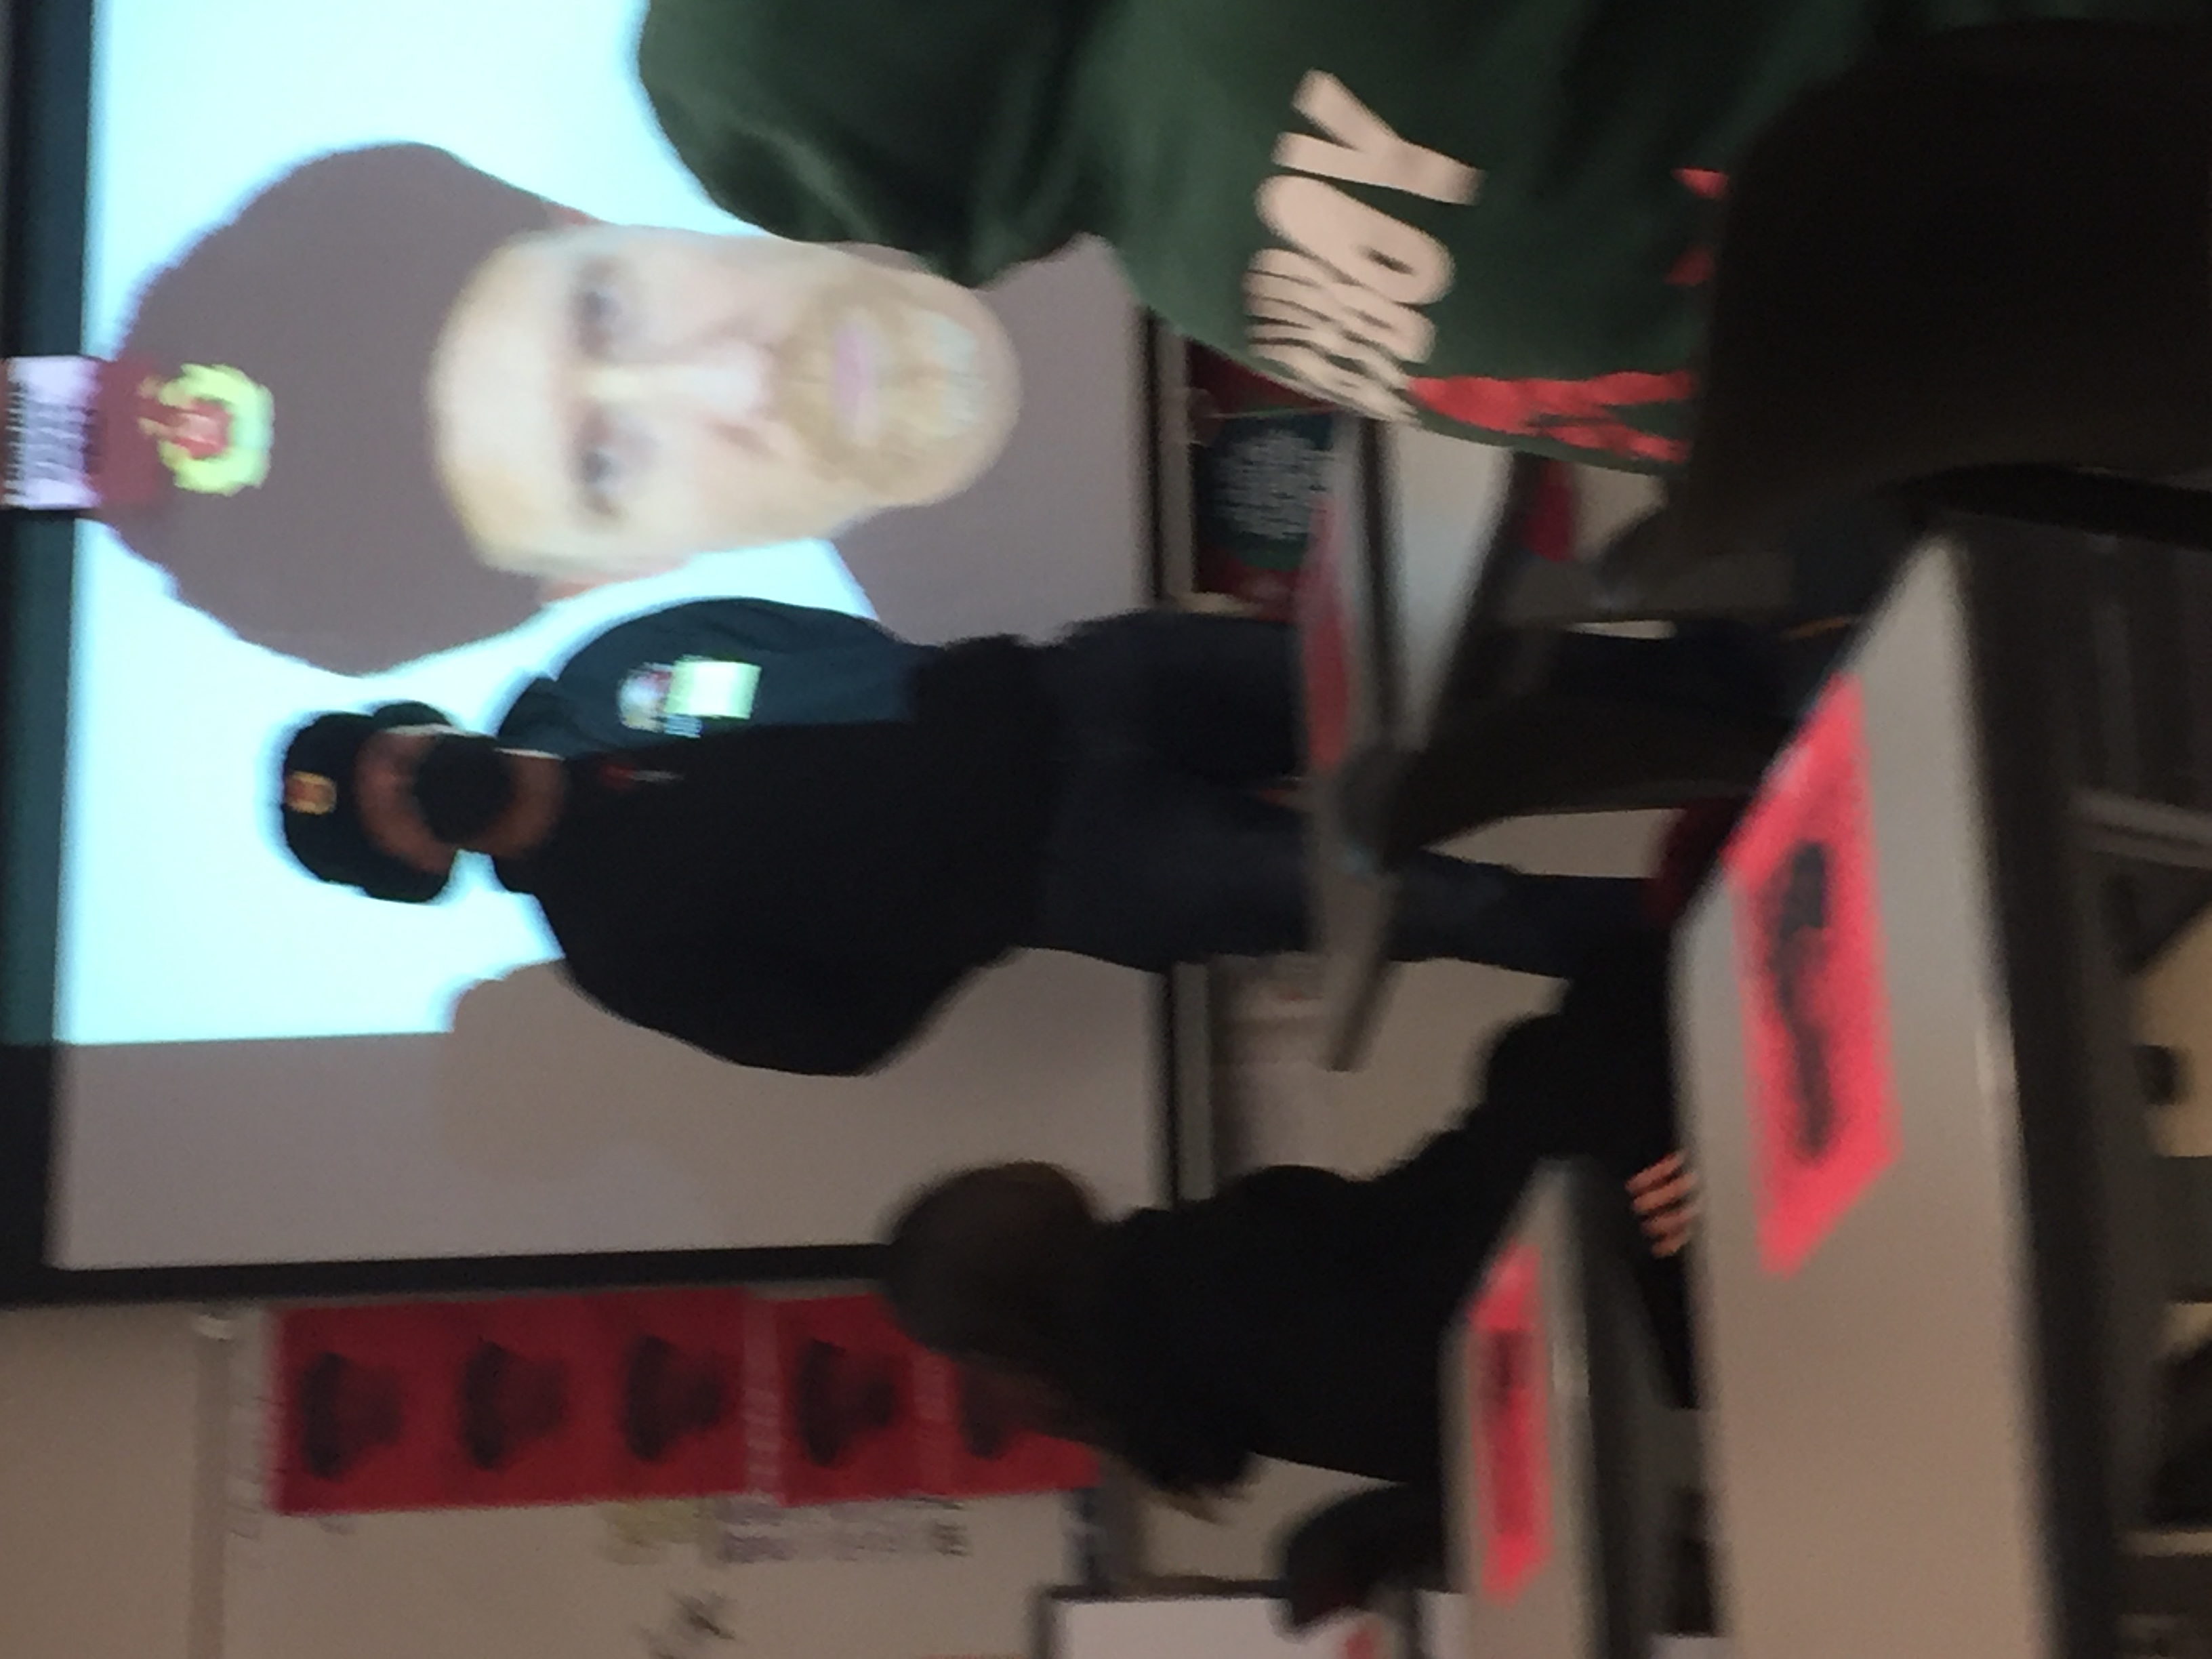
\includegraphics[width=90mm, angle=270]{LAST}}
 \caption{\label{MIDDLE}\small{Disgusting imagery containing the face and jawline of Mr.Kakes. Proof of his totalitarian rule }}
 \end{minipage}
 \end{center}
 \end{figure}


\subsection*{Agriculture and ur mom(Kidding just ur mom :) )}

\3

According to Mr.Kakes the agriculture industry of Kakesland is currently booming, as it always is according to Mr.Kakes. There are apparently abundant amounts of crops, tools to harvest said crops and machines to process them. The revenue from agriculture has also skyrocketed. Kakesland profits a lot off of their agricultural trade. 

\newpage

 \begin{figure}[!hbt]
 \begin{center}
 \begin{minipage}{0.85\textwidth}
 \centering{
\includegraphics[width=10mm, angle=0]{MEME}}
 \caption{\label{MEME}\small{The only image of the mother of Mr.Kakes }}
 \end{minipage}
 \end{center}
 \end{figure}

\section*{The Truth!}

While Mr.Kakes profits off of his false, and disgusting lies the truth must prevail. Artists in the \Kakes aren't celebrated, they are persecuted for not constantly praising their "Glorious" leader Mr.Kakes. All belief systems are banned except atheism, thus artists are not allowed to thrive and think about their own cultures. The political landscape of Kakesland, is indeed a muddy battlefield. The only allowed political party, is the one of Mr.Kakes. All votes must go to him, and ONLY him \&\ his party. The sole ruling class commits many atrocities such as murder, violence \&\ using the police to terrorize its citizens and stop reporters such as myself to gain the real truth. And the truth is that Kakesland is one of the most dangerous places to live in, due to the heavy persecution of its people to gratify the ego of its leader, Mr.Kakes. 

\section*{Conclusion}

\3

Ruling a country is difficult, that is to be expected. But one does not need to terrorize its citizens, and spread propaganda in favor of the ruling class. One does not need full totalitarian control over their constituents, for the sole reason of keeping your nation together. It should be illegal, and immediate action must be taken to punish such foolish and dangerous individuals who believe that ruling a country involves persecuting its citizens into submission. 

 \begin{figure}[!hbt]
 \begin{center}
 \begin{minipage}{0.85\textwidth}
 \centering{
\includegraphics[width=45mm, angle=0]{KAKES}}
 \caption{\label{KAKES}\small{ Mr. Kakes as an innocent and foolish young boy, yet to gain his destructive nature. }}
 \end{minipage}
 \end{center}
 \end{figure}

\3

I would advise anyone who is reading this article to call (505) 503-4455. This is the number of famed lawyer Saul Goodman, who will assist you in escaping the hellhole which we are forced to refer to as Kakesland. 







 
\end{document}

    